% Options for packages loaded elsewhere
\PassOptionsToPackage{unicode}{hyperref}
\PassOptionsToPackage{hyphens}{url}
%
\documentclass[
]{article}
\usepackage{amsmath,amssymb}
\usepackage{iftex}
\ifPDFTeX
  \usepackage[T1]{fontenc}
  \usepackage[utf8]{inputenc}
  \usepackage{textcomp} % provide euro and other symbols
\else % if luatex or xetex
  \usepackage{unicode-math} % this also loads fontspec
  \defaultfontfeatures{Scale=MatchLowercase}
  \defaultfontfeatures[\rmfamily]{Ligatures=TeX,Scale=1}
\fi
\usepackage{lmodern}
\ifPDFTeX\else
  % xetex/luatex font selection
\fi
% Use upquote if available, for straight quotes in verbatim environments
\IfFileExists{upquote.sty}{\usepackage{upquote}}{}
\IfFileExists{microtype.sty}{% use microtype if available
  \usepackage[]{microtype}
  \UseMicrotypeSet[protrusion]{basicmath} % disable protrusion for tt fonts
}{}
\makeatletter
\@ifundefined{KOMAClassName}{% if non-KOMA class
  \IfFileExists{parskip.sty}{%
    \usepackage{parskip}
  }{% else
    \setlength{\parindent}{0pt}
    \setlength{\parskip}{6pt plus 2pt minus 1pt}}
}{% if KOMA class
  \KOMAoptions{parskip=half}}
\makeatother
\usepackage{xcolor}
\usepackage[margin=1in]{geometry}
\usepackage{color}
\usepackage{fancyvrb}
\newcommand{\VerbBar}{|}
\newcommand{\VERB}{\Verb[commandchars=\\\{\}]}
\DefineVerbatimEnvironment{Highlighting}{Verbatim}{commandchars=\\\{\}}
% Add ',fontsize=\small' for more characters per line
\usepackage{framed}
\definecolor{shadecolor}{RGB}{248,248,248}
\newenvironment{Shaded}{\begin{snugshade}}{\end{snugshade}}
\newcommand{\AlertTok}[1]{\textcolor[rgb]{0.94,0.16,0.16}{#1}}
\newcommand{\AnnotationTok}[1]{\textcolor[rgb]{0.56,0.35,0.01}{\textbf{\textit{#1}}}}
\newcommand{\AttributeTok}[1]{\textcolor[rgb]{0.13,0.29,0.53}{#1}}
\newcommand{\BaseNTok}[1]{\textcolor[rgb]{0.00,0.00,0.81}{#1}}
\newcommand{\BuiltInTok}[1]{#1}
\newcommand{\CharTok}[1]{\textcolor[rgb]{0.31,0.60,0.02}{#1}}
\newcommand{\CommentTok}[1]{\textcolor[rgb]{0.56,0.35,0.01}{\textit{#1}}}
\newcommand{\CommentVarTok}[1]{\textcolor[rgb]{0.56,0.35,0.01}{\textbf{\textit{#1}}}}
\newcommand{\ConstantTok}[1]{\textcolor[rgb]{0.56,0.35,0.01}{#1}}
\newcommand{\ControlFlowTok}[1]{\textcolor[rgb]{0.13,0.29,0.53}{\textbf{#1}}}
\newcommand{\DataTypeTok}[1]{\textcolor[rgb]{0.13,0.29,0.53}{#1}}
\newcommand{\DecValTok}[1]{\textcolor[rgb]{0.00,0.00,0.81}{#1}}
\newcommand{\DocumentationTok}[1]{\textcolor[rgb]{0.56,0.35,0.01}{\textbf{\textit{#1}}}}
\newcommand{\ErrorTok}[1]{\textcolor[rgb]{0.64,0.00,0.00}{\textbf{#1}}}
\newcommand{\ExtensionTok}[1]{#1}
\newcommand{\FloatTok}[1]{\textcolor[rgb]{0.00,0.00,0.81}{#1}}
\newcommand{\FunctionTok}[1]{\textcolor[rgb]{0.13,0.29,0.53}{\textbf{#1}}}
\newcommand{\ImportTok}[1]{#1}
\newcommand{\InformationTok}[1]{\textcolor[rgb]{0.56,0.35,0.01}{\textbf{\textit{#1}}}}
\newcommand{\KeywordTok}[1]{\textcolor[rgb]{0.13,0.29,0.53}{\textbf{#1}}}
\newcommand{\NormalTok}[1]{#1}
\newcommand{\OperatorTok}[1]{\textcolor[rgb]{0.81,0.36,0.00}{\textbf{#1}}}
\newcommand{\OtherTok}[1]{\textcolor[rgb]{0.56,0.35,0.01}{#1}}
\newcommand{\PreprocessorTok}[1]{\textcolor[rgb]{0.56,0.35,0.01}{\textit{#1}}}
\newcommand{\RegionMarkerTok}[1]{#1}
\newcommand{\SpecialCharTok}[1]{\textcolor[rgb]{0.81,0.36,0.00}{\textbf{#1}}}
\newcommand{\SpecialStringTok}[1]{\textcolor[rgb]{0.31,0.60,0.02}{#1}}
\newcommand{\StringTok}[1]{\textcolor[rgb]{0.31,0.60,0.02}{#1}}
\newcommand{\VariableTok}[1]{\textcolor[rgb]{0.00,0.00,0.00}{#1}}
\newcommand{\VerbatimStringTok}[1]{\textcolor[rgb]{0.31,0.60,0.02}{#1}}
\newcommand{\WarningTok}[1]{\textcolor[rgb]{0.56,0.35,0.01}{\textbf{\textit{#1}}}}
\usepackage{graphicx}
\makeatletter
\def\maxwidth{\ifdim\Gin@nat@width>\linewidth\linewidth\else\Gin@nat@width\fi}
\def\maxheight{\ifdim\Gin@nat@height>\textheight\textheight\else\Gin@nat@height\fi}
\makeatother
% Scale images if necessary, so that they will not overflow the page
% margins by default, and it is still possible to overwrite the defaults
% using explicit options in \includegraphics[width, height, ...]{}
\setkeys{Gin}{width=\maxwidth,height=\maxheight,keepaspectratio}
% Set default figure placement to htbp
\makeatletter
\def\fps@figure{htbp}
\makeatother
\setlength{\emergencystretch}{3em} % prevent overfull lines
\providecommand{\tightlist}{%
  \setlength{\itemsep}{0pt}\setlength{\parskip}{0pt}}
\setcounter{secnumdepth}{-\maxdimen} % remove section numbering
\ifLuaTeX
  \usepackage{selnolig}  % disable illegal ligatures
\fi
\IfFileExists{bookmark.sty}{\usepackage{bookmark}}{\usepackage{hyperref}}
\IfFileExists{xurl.sty}{\usepackage{xurl}}{} % add URL line breaks if available
\urlstyle{same}
\hypersetup{
  pdftitle={Lab assignment 1: t-tests, linear regression, analyzing lexical decision task},
  pdfauthor={INFOMEPL},
  hidelinks,
  pdfcreator={LaTeX via pandoc}}

\title{Lab assignment 1: t-tests, linear regression, analyzing lexical
decision task}
\author{INFOMEPL}
\date{Deadline: Tuesday, February 27}

\begin{document}
\maketitle

\begin{Shaded}
\begin{Highlighting}[]
\FunctionTok{library}\NormalTok{(dplyr)}
\end{Highlighting}
\end{Shaded}

\begin{verbatim}
## 
## Attaching package: 'dplyr'
\end{verbatim}

\begin{verbatim}
## The following objects are masked from 'package:stats':
## 
##     filter, lag
\end{verbatim}

\begin{verbatim}
## The following objects are masked from 'package:base':
## 
##     intersect, setdiff, setequal, union
\end{verbatim}

\begin{Shaded}
\begin{Highlighting}[]
\FunctionTok{library}\NormalTok{(ggplot2)}
\NormalTok{itemdata }\OtherTok{\textless{}{-}} \FunctionTok{read.csv}\NormalTok{(}\StringTok{"MALD1\_SelectedItemData.csv"}\NormalTok{, }\AttributeTok{sep=}\StringTok{"}\SpecialCharTok{\textbackslash{}t}\StringTok{"}\NormalTok{)}
\NormalTok{responsedata }\OtherTok{\textless{}{-}} \FunctionTok{read.csv}\NormalTok{(}\StringTok{"MALD1\_SelectedResponseData.csv"}\NormalTok{, }\AttributeTok{sep=}\StringTok{"}\SpecialCharTok{\textbackslash{}t}\StringTok{"}\NormalTok{)}
\end{Highlighting}
\end{Shaded}

\hypertarget{q1-merge-data-and-report-basic-information}{%
\subsubsection{Q1: Merge data and report basic
information}\label{q1-merge-data-and-report-basic-information}}

Merge the two data frames (responsedata and itemdata) into one data
frame. Afterwards, report descriptive summaries for the whole dataset
and also separately for Subjects 15351, 16854 and 170373. Report
summaries of the following measures:

\begin{enumerate}
\def\labelenumi{\arabic{enumi}.}
\tightlist
\item
  Reaction times (RT)
\item
  Frequencies (use FreqCOCAspok, which is a spoken corpus of American
  English).
\item
  RT for words and pseudowords separately. Use the variable IsWord: when
  it is TRUE, the word is a real word, when it is FALSE it is a
  pseudoword.
\end{enumerate}

For descriptive summaries it is enough you report means and spread of
data - e.g., variances or standard deviations, or just a range of data.
You can also provide histograms (for example, by replicating the code we
have above; for RTs this is already done).

\begin{Shaded}
\begin{Highlighting}[]
\CommentTok{\# Merge data frames by item column which belongs to both data frames}
\NormalTok{merged\_data }\OtherTok{\textless{}{-}} \FunctionTok{merge}\NormalTok{(responsedata, itemdata, }\AttributeTok{by =} \StringTok{"Item"}\NormalTok{)}


\CommentTok{\# Overall descriptive summaries using range function to only get 1 row per summaries group}
\NormalTok{overall\_summaries }\OtherTok{\textless{}{-}}\NormalTok{ merged\_data }\SpecialCharTok{\%\textgreater{}\%}
  \FunctionTok{summarise}\NormalTok{(}
    \AttributeTok{MeanRT =} \FunctionTok{mean}\NormalTok{(RT, }\AttributeTok{na.rm =} \ConstantTok{TRUE}\NormalTok{),}
    \AttributeTok{SdRT =} \FunctionTok{sd}\NormalTok{(RT, }\AttributeTok{na.rm =} \ConstantTok{TRUE}\NormalTok{),}
    \AttributeTok{MinRT =} \FunctionTok{min}\NormalTok{(RT, }\AttributeTok{na.rm =} \ConstantTok{TRUE}\NormalTok{),}
    \AttributeTok{MaxRT =} \FunctionTok{max}\NormalTok{(RT, }\AttributeTok{na.rm =} \ConstantTok{TRUE}\NormalTok{),}
    \AttributeTok{MeanFreqCOCAspok =} \FunctionTok{mean}\NormalTok{(FreqCOCAspok, }\AttributeTok{na.rm =} \ConstantTok{TRUE}\NormalTok{),}
    \AttributeTok{SdFreqCOCAspok =} \FunctionTok{sd}\NormalTok{(FreqCOCAspok, }\AttributeTok{na.rm =} \ConstantTok{TRUE}\NormalTok{),}
    \AttributeTok{MinFreqCOCAspok =} \FunctionTok{min}\NormalTok{(FreqCOCAspok, }\AttributeTok{na.rm =} \ConstantTok{TRUE}\NormalTok{),}
    \AttributeTok{MaxFreqCOCAspok =} \FunctionTok{max}\NormalTok{(FreqCOCAspok, }\AttributeTok{na.rm =} \ConstantTok{TRUE}\NormalTok{)}
\NormalTok{  )}

\CommentTok{\# RT for words and pseudowords}
\NormalTok{word\_pseudoword\_summary }\OtherTok{\textless{}{-}}\NormalTok{ merged\_data }\SpecialCharTok{\%\textgreater{}\%}
  \FunctionTok{group\_by}\NormalTok{(IsWord) }\SpecialCharTok{\%\textgreater{}\%}
  \FunctionTok{summarise}\NormalTok{(}
    \AttributeTok{MeanRT =} \FunctionTok{mean}\NormalTok{(RT, }\AttributeTok{na.rm =} \ConstantTok{TRUE}\NormalTok{),}
    \AttributeTok{SdRT =} \FunctionTok{sd}\NormalTok{(RT, }\AttributeTok{na.rm =} \ConstantTok{TRUE}\NormalTok{),}
    \AttributeTok{MinRT =} \FunctionTok{min}\NormalTok{(RT, }\AttributeTok{na.rm =} \ConstantTok{TRUE}\NormalTok{),}
    \AttributeTok{MaxRT =} \FunctionTok{max}\NormalTok{(RT, }\AttributeTok{na.rm =} \ConstantTok{TRUE}\NormalTok{)}
\NormalTok{  )}

\CommentTok{\# For specific subjects}
\NormalTok{subjects\_summary }\OtherTok{\textless{}{-}}\NormalTok{ merged\_data }\SpecialCharTok{\%\textgreater{}\%}
  \FunctionTok{filter}\NormalTok{(Subject }\SpecialCharTok{\%in\%} \FunctionTok{c}\NormalTok{(}\DecValTok{15351}\NormalTok{, }\DecValTok{16854}\NormalTok{, }\DecValTok{170373}\NormalTok{)) }\SpecialCharTok{\%\textgreater{}\%}
  \FunctionTok{group\_by}\NormalTok{(Subject) }\SpecialCharTok{\%\textgreater{}\%}
  \FunctionTok{summarise}\NormalTok{(}
    \AttributeTok{MeanRT =} \FunctionTok{mean}\NormalTok{(RT, }\AttributeTok{na.rm =} \ConstantTok{TRUE}\NormalTok{),}
    \AttributeTok{SdRT =} \FunctionTok{sd}\NormalTok{(RT, }\AttributeTok{na.rm =} \ConstantTok{TRUE}\NormalTok{),}
    \AttributeTok{MinRT =} \FunctionTok{min}\NormalTok{(RT, }\AttributeTok{na.rm =} \ConstantTok{TRUE}\NormalTok{),}
    \AttributeTok{MaxRT =} \FunctionTok{max}\NormalTok{(RT, }\AttributeTok{na.rm =} \ConstantTok{TRUE}\NormalTok{),}
    \AttributeTok{MeanFreqCOCAspok =} \FunctionTok{mean}\NormalTok{(FreqCOCAspok, }\AttributeTok{na.rm =} \ConstantTok{TRUE}\NormalTok{),}
    \AttributeTok{SdFreqCOCAspok =} \FunctionTok{sd}\NormalTok{(FreqCOCAspok, }\AttributeTok{na.rm =} \ConstantTok{TRUE}\NormalTok{),}
    \AttributeTok{MinFreqCOCAspok =} \FunctionTok{min}\NormalTok{(FreqCOCAspok, }\AttributeTok{na.rm =} \ConstantTok{TRUE}\NormalTok{),}
    \AttributeTok{MaxFreqCOCAspok =} \FunctionTok{max}\NormalTok{(FreqCOCAspok, }\AttributeTok{na.rm =} \ConstantTok{TRUE}\NormalTok{)}
\NormalTok{  )}

\CommentTok{\# View the data frames}
\FunctionTok{View}\NormalTok{(overall\_summaries)}
\FunctionTok{View}\NormalTok{(subjects\_summary)}
\FunctionTok{View}\NormalTok{(word\_pseudoword\_summary)}

\CommentTok{\# Histogram for Response times (overall)}
\FunctionTok{ggplot}\NormalTok{(merged\_data, }\FunctionTok{aes}\NormalTok{(}\AttributeTok{x =}\NormalTok{ RT)) }\SpecialCharTok{+}
  \FunctionTok{geom\_histogram}\NormalTok{(}\AttributeTok{binwidth =} \DecValTok{100}\NormalTok{, }\AttributeTok{fill =} \StringTok{"blue"}\NormalTok{, }\AttributeTok{color =} \StringTok{"black"}\NormalTok{) }\SpecialCharTok{+}
  \FunctionTok{labs}\NormalTok{(}\AttributeTok{title =} \StringTok{"Histogram of Reaction Times"}\NormalTok{, }\AttributeTok{x =} \StringTok{"Reaction Time (ms)"}\NormalTok{, }\AttributeTok{y =} \StringTok{"Frequency"}\NormalTok{) }\SpecialCharTok{+}
  \FunctionTok{theme\_minimal}\NormalTok{()}
\end{Highlighting}
\end{Shaded}

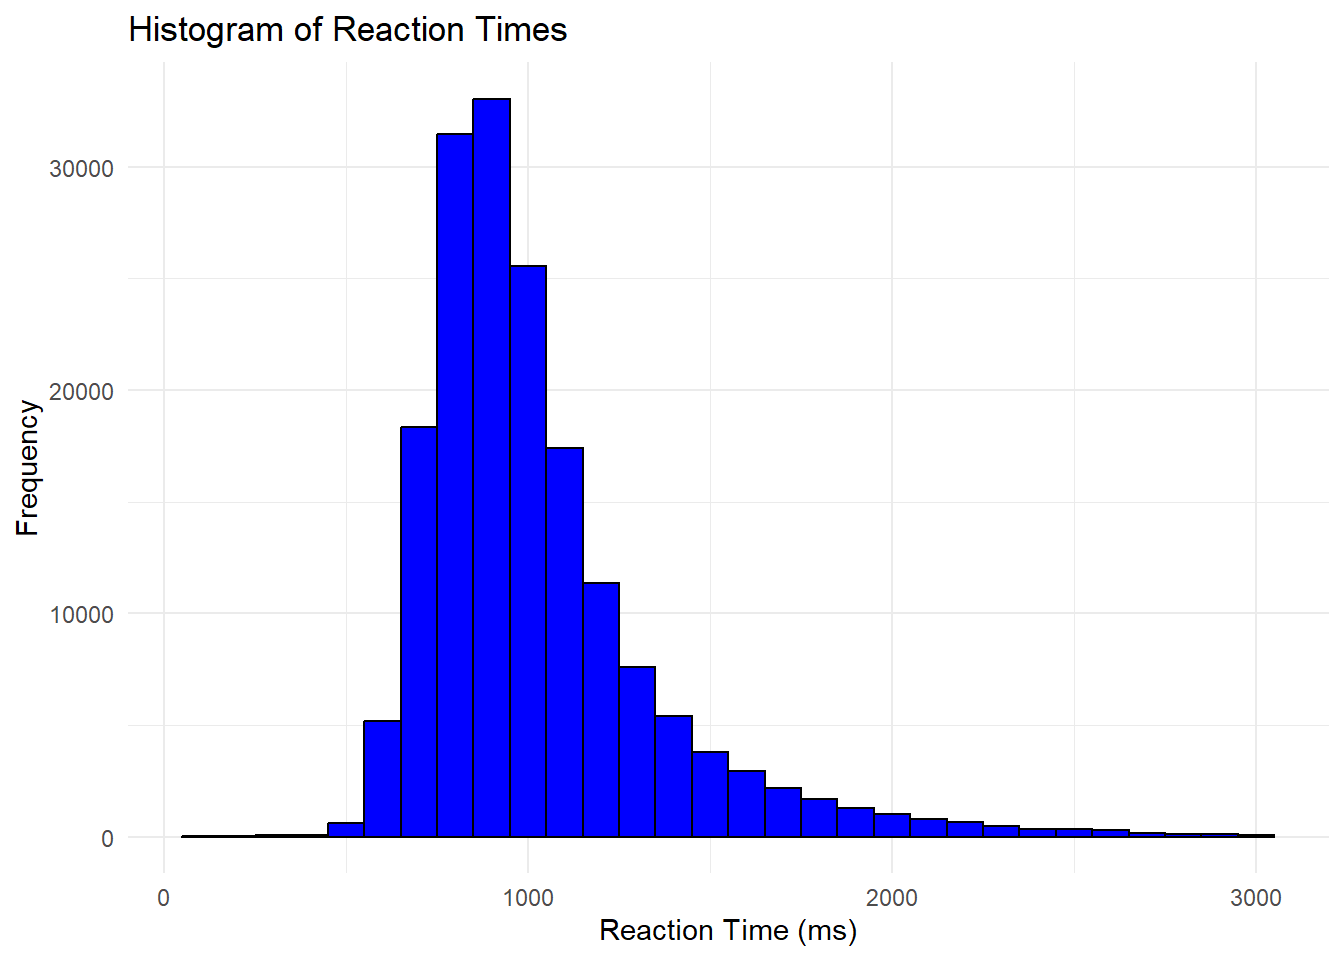
\includegraphics{assignment1_final_files/figure-latex/unnamed-chunk-2-1.pdf}

\hypertarget{q2-implement-cohens-d-and-the-calculation-of-t-values}{%
\subsubsection{Q2: Implement Cohen's d and the calculation of t
values}\label{q2-implement-cohens-d-and-the-calculation-of-t-values}}

In answering this question, you are not allowed to use any R packages or
R functions that implement Cohen's d or the calculation of t-tests.
However, you can use such packages (for example, effsize for Cohen's d
and t.test for t-values) to double-check that your function works
correctly. In doing so, be careful - some implementations might slightly
differ wrt how they calculate \(s\), so you might not get exactly
identical numbers. This is another reason why you should not just rely
on another package in your answer. If you check, say, stackoverflow or
use an AI tool like ChatGPT, you should also be careful -- there are
various ways of implementing Cohen's \(d\) and \(t\) calculation and not
all are equivalent to what we do here.

First, implement Cohen's \(d\) as a function in R. That is, you have to
fill in the body of the function (what is put in as\ldots) that you have
here below. As said above, it is enough to implement the simplified
version (one in which the length of \(x_1\) and \(x_2\) is the same).

\begin{Shaded}
\begin{Highlighting}[]
\CommentTok{\# n1 and n2 should be equal}
\NormalTok{cohend }\OtherTok{\textless{}{-}} \ControlFlowTok{function}\NormalTok{(x1, x2) \{}
\NormalTok{  mean\_x1 }\OtherTok{\textless{}{-}} \FunctionTok{mean}\NormalTok{(x1)}
\NormalTok{  mean\_x2 }\OtherTok{\textless{}{-}} \FunctionTok{mean}\NormalTok{(x2)}
\NormalTok{  s }\OtherTok{\textless{}{-}} \FunctionTok{sqrt}\NormalTok{((}\FunctionTok{length}\NormalTok{(x1) }\SpecialCharTok{{-}} \DecValTok{1}\NormalTok{) }\SpecialCharTok{*}\NormalTok{ (}\FunctionTok{var}\NormalTok{(x1) }\SpecialCharTok{+} \FunctionTok{var}\NormalTok{(x2)) }\SpecialCharTok{/}\NormalTok{ (}\DecValTok{2}\SpecialCharTok{*}\FunctionTok{length}\NormalTok{(x1) }\SpecialCharTok{{-}} \DecValTok{2}\NormalTok{))}
\NormalTok{  d }\OtherTok{\textless{}{-}}\NormalTok{ (mean\_x1 }\SpecialCharTok{{-}}\NormalTok{ mean\_x2) }\SpecialCharTok{/}\NormalTok{ s}
  \FunctionTok{return}\NormalTok{(d)}
\NormalTok{\}}
\end{Highlighting}
\end{Shaded}

After the implementation, test your function and report collected
Cohen's \(d\) on four cases discussed below. Along with that, report
whether the effect size is small, medium or large (\(|d|<0.5\) is small,
\(|d|<0.8\) is medium, above that is large).

\begin{enumerate}
\def\labelenumi{\arabic{enumi}.}
\tightlist
\item
  RTs for words and pseudowords for Subject numbered 15351.
\item
  RTs for words and pseudowords for Subject numbered 16854.
\item
  RTs for words and pseudowords for Subject numbered 170373.
\item
  RTs for all words and pseudowords.
\item
  RTs for the two vectors provided below as word\_15292 and
  pseudoword\_15292 (these are a few selected responses to words and
  pseudowords from subject 15292).
\end{enumerate}

\begin{Shaded}
\begin{Highlighting}[]
\NormalTok{subject\_number }\OtherTok{\textless{}{-}} \DecValTok{15351}

\CommentTok{\# Get the response time for the word and pseudowords}
\NormalTok{words\_rt }\OtherTok{\textless{}{-}}\NormalTok{ merged\_data }\SpecialCharTok{\%\textgreater{}\%}
  \FunctionTok{filter}\NormalTok{(Subject }\SpecialCharTok{==}\NormalTok{ subject\_number, IsWord }\SpecialCharTok{==} \ConstantTok{TRUE}\NormalTok{) }\SpecialCharTok{\%\textgreater{}\%}
  \FunctionTok{pull}\NormalTok{(RT)}

\NormalTok{pseudowords\_rt }\OtherTok{\textless{}{-}}\NormalTok{ merged\_data }\SpecialCharTok{\%\textgreater{}\%}
  \FunctionTok{filter}\NormalTok{(Subject }\SpecialCharTok{==}\NormalTok{ subject\_number, IsWord }\SpecialCharTok{==} \ConstantTok{FALSE}\NormalTok{) }\SpecialCharTok{\%\textgreater{}\%}
  \FunctionTok{pull}\NormalTok{(RT)}

\NormalTok{effect\_size\_classification }\OtherTok{\textless{}{-}} \ControlFlowTok{function}\NormalTok{(d) \{}
  \ControlFlowTok{if}\NormalTok{(}\FunctionTok{abs}\NormalTok{(d) }\SpecialCharTok{\textless{}} \FloatTok{0.5}\NormalTok{) \{}
    \FunctionTok{return}\NormalTok{(}\StringTok{"small"}\NormalTok{)}
\NormalTok{  \} }\ControlFlowTok{else} \ControlFlowTok{if}\NormalTok{(}\FunctionTok{abs}\NormalTok{(d) }\SpecialCharTok{\textless{}} \FloatTok{0.8}\NormalTok{) \{}
    \FunctionTok{return}\NormalTok{(}\StringTok{"medium"}\NormalTok{)}
\NormalTok{  \} }\ControlFlowTok{else}\NormalTok{ \{}
    \FunctionTok{return}\NormalTok{(}\StringTok{"large"}\NormalTok{)}
\NormalTok{  \}}
\NormalTok{\}}


\CommentTok{\# 1.Calculate Cohen\textquotesingle{}s d for 15351}
\CommentTok{\# "Cohen\textquotesingle{}s d for subject 15351 is {-}1.39943111730686 . Effect size is large ."}
\NormalTok{subject\_number }\OtherTok{\textless{}{-}} \DecValTok{15351}

\NormalTok{words\_rt }\OtherTok{\textless{}{-}}\NormalTok{ merged\_data }\SpecialCharTok{\%\textgreater{}\%}
  \FunctionTok{filter}\NormalTok{(Subject }\SpecialCharTok{==}\NormalTok{ subject\_number, IsWord }\SpecialCharTok{==} \ConstantTok{TRUE}\NormalTok{) }\SpecialCharTok{\%\textgreater{}\%}
  \FunctionTok{pull}\NormalTok{(RT)}

\NormalTok{pseudowords\_rt }\OtherTok{\textless{}{-}}\NormalTok{ merged\_data }\SpecialCharTok{\%\textgreater{}\%}
  \FunctionTok{filter}\NormalTok{(Subject }\SpecialCharTok{==}\NormalTok{ subject\_number, IsWord }\SpecialCharTok{==} \ConstantTok{FALSE}\NormalTok{) }\SpecialCharTok{\%\textgreater{}\%}
  \FunctionTok{pull}\NormalTok{(RT)}

\NormalTok{d\_value }\OtherTok{\textless{}{-}} \FunctionTok{cohend}\NormalTok{(words\_rt, pseudowords\_rt)}
\NormalTok{effect\_size }\OtherTok{\textless{}{-}} \FunctionTok{effect\_size\_classification}\NormalTok{(d\_value)}

\FunctionTok{print}\NormalTok{(}\FunctionTok{paste}\NormalTok{(}\StringTok{"Cohen\textquotesingle{}s d for subject"}\NormalTok{, subject\_number, }\StringTok{"is"}\NormalTok{, d\_value, }\StringTok{". Effect size is"}\NormalTok{, effect\_size, }\StringTok{"."}\NormalTok{))}
\end{Highlighting}
\end{Shaded}

\begin{verbatim}
## [1] "Cohen's d for subject 15351 is -1.39943111730686 . Effect size is large ."
\end{verbatim}

\begin{Shaded}
\begin{Highlighting}[]
\CommentTok{\# 2.Calculate Cohen\textquotesingle{}s d for 16854}
\CommentTok{\#  "Cohen\textquotesingle{}s d for subject 16854 is {-}0.171013812364667 . Effect size is small ."}
\NormalTok{subject\_number }\OtherTok{\textless{}{-}} \DecValTok{16854}

\NormalTok{words\_rt }\OtherTok{\textless{}{-}}\NormalTok{ merged\_data }\SpecialCharTok{\%\textgreater{}\%}
  \FunctionTok{filter}\NormalTok{(Subject }\SpecialCharTok{==}\NormalTok{ subject\_number, IsWord }\SpecialCharTok{==} \ConstantTok{TRUE}\NormalTok{) }\SpecialCharTok{\%\textgreater{}\%}
  \FunctionTok{pull}\NormalTok{(RT)}

\NormalTok{pseudowords\_rt }\OtherTok{\textless{}{-}}\NormalTok{ merged\_data }\SpecialCharTok{\%\textgreater{}\%}
  \FunctionTok{filter}\NormalTok{(Subject }\SpecialCharTok{==}\NormalTok{ subject\_number, IsWord }\SpecialCharTok{==} \ConstantTok{FALSE}\NormalTok{) }\SpecialCharTok{\%\textgreater{}\%}
  \FunctionTok{pull}\NormalTok{(RT)}

\NormalTok{d\_value }\OtherTok{\textless{}{-}} \FunctionTok{cohend}\NormalTok{(words\_rt, pseudowords\_rt)}
\NormalTok{effect\_size }\OtherTok{\textless{}{-}} \FunctionTok{effect\_size\_classification}\NormalTok{(d\_value)}

\FunctionTok{print}\NormalTok{(}\FunctionTok{paste}\NormalTok{(}\StringTok{"Cohen\textquotesingle{}s d for subject"}\NormalTok{, subject\_number, }\StringTok{"is"}\NormalTok{, d\_value, }\StringTok{". Effect size is"}\NormalTok{, effect\_size, }\StringTok{"."}\NormalTok{))}
\end{Highlighting}
\end{Shaded}

\begin{verbatim}
## [1] "Cohen's d for subject 16854 is -0.171013812364667 . Effect size is small ."
\end{verbatim}

\begin{Shaded}
\begin{Highlighting}[]
\CommentTok{\# 3. Calculate Cohen\textquotesingle{}s d for 170373}
\CommentTok{\# "Cohen\textquotesingle{}s d for subject 170373 is {-}0.343143399184897 . Effect size is small ."}

\NormalTok{subject\_number }\OtherTok{\textless{}{-}} \DecValTok{170373}

\NormalTok{words\_rt }\OtherTok{\textless{}{-}}\NormalTok{ merged\_data }\SpecialCharTok{\%\textgreater{}\%}
  \FunctionTok{filter}\NormalTok{(Subject }\SpecialCharTok{==}\NormalTok{ subject\_number, IsWord }\SpecialCharTok{==} \ConstantTok{TRUE}\NormalTok{) }\SpecialCharTok{\%\textgreater{}\%}
  \FunctionTok{pull}\NormalTok{(RT)}

\NormalTok{pseudowords\_rt }\OtherTok{\textless{}{-}}\NormalTok{ merged\_data }\SpecialCharTok{\%\textgreater{}\%}
  \FunctionTok{filter}\NormalTok{(Subject }\SpecialCharTok{==}\NormalTok{ subject\_number, IsWord }\SpecialCharTok{==} \ConstantTok{FALSE}\NormalTok{) }\SpecialCharTok{\%\textgreater{}\%}
  \FunctionTok{pull}\NormalTok{(RT)}

\NormalTok{d\_value }\OtherTok{\textless{}{-}} \FunctionTok{cohend}\NormalTok{(words\_rt, pseudowords\_rt)}
\NormalTok{effect\_size }\OtherTok{\textless{}{-}} \FunctionTok{effect\_size\_classification}\NormalTok{(d\_value)}

\FunctionTok{print}\NormalTok{(}\FunctionTok{paste}\NormalTok{(}\StringTok{"Cohen\textquotesingle{}s d for subject"}\NormalTok{, subject\_number, }\StringTok{"is"}\NormalTok{, d\_value, }\StringTok{". Effect size is"}\NormalTok{, effect\_size, }\StringTok{"."}\NormalTok{))}
\end{Highlighting}
\end{Shaded}

\begin{verbatim}
## [1] "Cohen's d for subject 170373 is -0.343143399184897 . Effect size is small ."
\end{verbatim}

\begin{Shaded}
\begin{Highlighting}[]
\CommentTok{\# 4.For all words and pseudowords}
\CommentTok{\# "Cohen\textquotesingle{}s d for all words and pseudowords 170373 is {-}0.410810089564915 . Effect size is small ."}
\NormalTok{words\_rt }\OtherTok{\textless{}{-}}\NormalTok{ merged\_data }\SpecialCharTok{\%\textgreater{}\%}
  \FunctionTok{filter}\NormalTok{(IsWord }\SpecialCharTok{==} \ConstantTok{TRUE}\NormalTok{) }\SpecialCharTok{\%\textgreater{}\%}
  \FunctionTok{pull}\NormalTok{(RT)}

\NormalTok{pseudowords\_rt }\OtherTok{\textless{}{-}}\NormalTok{ merged\_data }\SpecialCharTok{\%\textgreater{}\%}
  \FunctionTok{filter}\NormalTok{( IsWord }\SpecialCharTok{==} \ConstantTok{FALSE}\NormalTok{) }\SpecialCharTok{\%\textgreater{}\%}
  \FunctionTok{pull}\NormalTok{(RT)}

\NormalTok{d\_value }\OtherTok{\textless{}{-}} \FunctionTok{cohend}\NormalTok{(words\_rt, pseudowords\_rt)}
\NormalTok{effect\_size }\OtherTok{\textless{}{-}} \FunctionTok{effect\_size\_classification}\NormalTok{(d\_value)}

\FunctionTok{print}\NormalTok{(}\FunctionTok{paste}\NormalTok{(}\StringTok{"Cohen\textquotesingle{}s d for all words and pseudowords"}\NormalTok{, subject\_number, }\StringTok{"is"}\NormalTok{, d\_value, }\StringTok{". Effect size is"}\NormalTok{, effect\_size, }\StringTok{"."}\NormalTok{))}
\end{Highlighting}
\end{Shaded}

\begin{verbatim}
## [1] "Cohen's d for all words and pseudowords 170373 is -0.410810089564973 . Effect size is small ."
\end{verbatim}

\begin{Shaded}
\begin{Highlighting}[]
\CommentTok{\# 5.Calculate Cohen\textquotesingle{}s d for the 2 vectors}

\NormalTok{subject\_number }\OtherTok{\textless{}{-}} \DecValTok{15292}
\CommentTok{\#  "Cohen\textquotesingle{}s d for subject 15292 is 0 . Effect size is small ."}
\NormalTok{word\_15292 }\OtherTok{\textless{}{-}} \FunctionTok{c}\NormalTok{(}\DecValTok{2206}\NormalTok{, }\DecValTok{1583}\NormalTok{, }\DecValTok{1154}\NormalTok{, }\DecValTok{1010}\NormalTok{,  }\DecValTok{865}\NormalTok{,  }\DecValTok{931}\NormalTok{, }\DecValTok{1129}\NormalTok{,  }\DecValTok{683}\NormalTok{,  }\DecValTok{820}\NormalTok{, }\DecValTok{1132}\NormalTok{, }\DecValTok{1049}\NormalTok{, }\DecValTok{1211}\NormalTok{, }\DecValTok{1261}\NormalTok{, }\DecValTok{957}\NormalTok{, }\DecValTok{1058}\NormalTok{,  }\DecValTok{790}\NormalTok{,  }\DecValTok{851}\NormalTok{, }\DecValTok{1908}\NormalTok{, }\DecValTok{1504}\NormalTok{, }\DecValTok{1400}\NormalTok{,  }\DecValTok{924}\NormalTok{)}

\NormalTok{pseudoword\_15292 }\OtherTok{\textless{}{-}} \FunctionTok{c}\NormalTok{(}\DecValTok{677}\NormalTok{,  }\DecValTok{949}\NormalTok{,  }\DecValTok{889}\NormalTok{,  }\DecValTok{881}\NormalTok{,  }\DecValTok{917}\NormalTok{,  }\DecValTok{769}\NormalTok{,  }\DecValTok{772}\NormalTok{,  }\DecValTok{922}\NormalTok{, }\DecValTok{1944}\NormalTok{,  }\DecValTok{881}\NormalTok{,  }\DecValTok{976}\NormalTok{, }\DecValTok{1087}\NormalTok{, }\DecValTok{1252}\NormalTok{,  }\DecValTok{914}\NormalTok{, }\DecValTok{1277}\NormalTok{,  }\DecValTok{825}\NormalTok{, }\DecValTok{1295}\NormalTok{, }\DecValTok{1336}\NormalTok{,  }\DecValTok{788}\NormalTok{,  }\DecValTok{885}\NormalTok{,  }\DecValTok{932}\NormalTok{)}
\NormalTok{d\_value }\OtherTok{\textless{}{-}} \FunctionTok{cohend}\NormalTok{(word\_15292, word\_15292)}
\NormalTok{effect\_size }\OtherTok{\textless{}{-}} \FunctionTok{effect\_size\_classification}\NormalTok{(d\_value)}

\FunctionTok{print}\NormalTok{(}\FunctionTok{paste}\NormalTok{(}\StringTok{"Cohen\textquotesingle{}s d for subject"}\NormalTok{, subject\_number, }\StringTok{"is"}\NormalTok{, d\_value, }\StringTok{". Effect size is"}\NormalTok{, effect\_size, }\StringTok{"."}\NormalTok{))}
\end{Highlighting}
\end{Shaded}

\begin{verbatim}
## [1] "Cohen's d for subject 15292 is 0 . Effect size is small ."
\end{verbatim}

Finally, implement the t-calculation as a function. That is, fill in the
body of this function (the same limitation that applied to Cohen's d
applies here -- you cannot use other packages or R functions like t.test
but you can consult AI tools or websites - and again, be careful if you
use that, because there are different versions of t-tests):

\begin{Shaded}
\begin{Highlighting}[]
\NormalTok{tcalculation }\OtherTok{\textless{}{-}} \ControlFlowTok{function}\NormalTok{(x1, x2) \{}
\NormalTok{  mean\_x1 }\OtherTok{\textless{}{-}} \FunctionTok{mean}\NormalTok{(x1)}
\NormalTok{  mean\_x2 }\OtherTok{\textless{}{-}} \FunctionTok{mean}\NormalTok{(x2)}
\NormalTok{  se }\OtherTok{\textless{}{-}} \FunctionTok{sqrt}\NormalTok{((}\FunctionTok{var}\NormalTok{(x1) }\SpecialCharTok{+} \FunctionTok{var}\NormalTok{(x2)) }\SpecialCharTok{/} \FunctionTok{length}\NormalTok{(x1))}
\NormalTok{  t }\OtherTok{\textless{}{-}}\NormalTok{ (mean\_x1 }\SpecialCharTok{{-}}\NormalTok{ mean\_x2) }\SpecialCharTok{/}\NormalTok{ se}

\NormalTok{\}}

\NormalTok{subject\_number }\OtherTok{\textless{}{-}} \DecValTok{15351}

\NormalTok{words\_rt }\OtherTok{\textless{}{-}}\NormalTok{ merged\_data }\SpecialCharTok{\%\textgreater{}\%}
  \FunctionTok{filter}\NormalTok{(Subject }\SpecialCharTok{==}\NormalTok{ subject\_number, IsWord }\SpecialCharTok{==} \ConstantTok{TRUE}\NormalTok{) }\SpecialCharTok{\%\textgreater{}\%}
  \FunctionTok{pull}\NormalTok{(RT)}

\NormalTok{pseudowords\_rt }\OtherTok{\textless{}{-}}\NormalTok{ merged\_data }\SpecialCharTok{\%\textgreater{}\%}
  \FunctionTok{filter}\NormalTok{(Subject }\SpecialCharTok{==}\NormalTok{ subject\_number, IsWord }\SpecialCharTok{==} \ConstantTok{FALSE}\NormalTok{) }\SpecialCharTok{\%\textgreater{}\%}
  \FunctionTok{pull}\NormalTok{(RT)}

\NormalTok{t\_value }\OtherTok{\textless{}{-}} \FunctionTok{tcalculation}\NormalTok{(words\_rt, pseudowords\_rt)}

\FunctionTok{print}\NormalTok{(}\FunctionTok{paste}\NormalTok{(}\StringTok{"1: T value d for subject"}\NormalTok{, subject\_number, }\StringTok{"is"}\NormalTok{, t\_value, }\StringTok{"."}\NormalTok{))}
\end{Highlighting}
\end{Shaded}

\begin{verbatim}
## [1] "1: T value d for subject 15351 is -19.5419920467928 ."
\end{verbatim}

\begin{Shaded}
\begin{Highlighting}[]
\CommentTok{\# T value for all words}
\NormalTok{words\_rt }\OtherTok{\textless{}{-}}\NormalTok{ merged\_data }\SpecialCharTok{\%\textgreater{}\%}
  \FunctionTok{filter}\NormalTok{(IsWord }\SpecialCharTok{==} \ConstantTok{TRUE}\NormalTok{) }\SpecialCharTok{\%\textgreater{}\%}
  \FunctionTok{pull}\NormalTok{(RT)}

\NormalTok{pseudowords\_rt }\OtherTok{\textless{}{-}}\NormalTok{ merged\_data }\SpecialCharTok{\%\textgreater{}\%}
  \FunctionTok{filter}\NormalTok{( IsWord }\SpecialCharTok{==} \ConstantTok{FALSE}\NormalTok{) }\SpecialCharTok{\%\textgreater{}\%}
  \FunctionTok{pull}\NormalTok{(RT)}

\NormalTok{t\_value }\OtherTok{\textless{}{-}} \FunctionTok{tcalculation}\NormalTok{(words\_rt, pseudowords\_rt)}

\FunctionTok{print}\NormalTok{(}\FunctionTok{paste}\NormalTok{(}\StringTok{"2: T value d for all words is"}\NormalTok{, t\_value, }\StringTok{"."}\NormalTok{))}
\end{Highlighting}
\end{Shaded}

\begin{verbatim}
## [1] "2: T value d for all words is -85.2814437314518 ."
\end{verbatim}

\begin{Shaded}
\begin{Highlighting}[]
\CommentTok{\# T value for specified vectors}
\NormalTok{word\_15292 }\OtherTok{\textless{}{-}} \FunctionTok{c}\NormalTok{(}\DecValTok{2206}\NormalTok{, }\DecValTok{1583}\NormalTok{, }\DecValTok{1154}\NormalTok{, }\DecValTok{1010}\NormalTok{,  }\DecValTok{865}\NormalTok{,  }\DecValTok{931}\NormalTok{, }\DecValTok{1129}\NormalTok{,  }\DecValTok{683}\NormalTok{,  }\DecValTok{820}\NormalTok{, }\DecValTok{1132}\NormalTok{, }\DecValTok{1049}\NormalTok{, }\DecValTok{1211}\NormalTok{, }\DecValTok{1261}\NormalTok{, }\DecValTok{957}\NormalTok{, }\DecValTok{1058}\NormalTok{,  }\DecValTok{790}\NormalTok{,  }\DecValTok{851}\NormalTok{, }\DecValTok{1908}\NormalTok{, }\DecValTok{1504}\NormalTok{, }\DecValTok{1400}\NormalTok{,  }\DecValTok{924}\NormalTok{)}

\NormalTok{pseudoword\_15292 }\OtherTok{\textless{}{-}} \FunctionTok{c}\NormalTok{(}\DecValTok{677}\NormalTok{,  }\DecValTok{949}\NormalTok{,  }\DecValTok{889}\NormalTok{,  }\DecValTok{881}\NormalTok{,  }\DecValTok{917}\NormalTok{,  }\DecValTok{769}\NormalTok{,  }\DecValTok{772}\NormalTok{,  }\DecValTok{922}\NormalTok{, }\DecValTok{1944}\NormalTok{,  }\DecValTok{881}\NormalTok{,  }\DecValTok{976}\NormalTok{, }\DecValTok{1087}\NormalTok{, }\DecValTok{1252}\NormalTok{,  }\DecValTok{914}\NormalTok{, }\DecValTok{1277}\NormalTok{,  }\DecValTok{825}\NormalTok{, }\DecValTok{1295}\NormalTok{, }\DecValTok{1336}\NormalTok{,  }\DecValTok{788}\NormalTok{,  }\DecValTok{885}\NormalTok{,  }\DecValTok{932}\NormalTok{)}

\NormalTok{t\_value }\OtherTok{\textless{}{-}} \FunctionTok{tcalculation}\NormalTok{(word\_15292, pseudoword\_15292)}

\FunctionTok{print}\NormalTok{(}\FunctionTok{paste}\NormalTok{(}\StringTok{"3: T value d for specified vectors is"}\NormalTok{, t\_value, }\StringTok{"."}\NormalTok{))}
\end{Highlighting}
\end{Shaded}

\begin{verbatim}
## [1] "3: T value d for specified vectors is 1.50136643517682 ."
\end{verbatim}

\begin{Shaded}
\begin{Highlighting}[]
\FunctionTok{print}\NormalTok{(}\FunctionTok{t.test}\NormalTok{(word\_15292, pseudoword\_15292,  }\AttributeTok{paired =} \ConstantTok{FALSE}\NormalTok{, }\AttributeTok{alternative =} \StringTok{"two.sided"}\NormalTok{))}
\end{Highlighting}
\end{Shaded}

\begin{verbatim}
## 
##  Welch Two Sample t-test
## 
## data:  word_15292 and pseudoword_15292
## t = 1.5014, df = 37.008, p-value = 0.1417
## alternative hypothesis: true difference in means is not equal to 0
## 95 percent confidence interval:
##  -54.23106 364.51678
## sample estimates:
## mean of x mean of y 
##  1163.143  1008.000
\end{verbatim}

Once the implementation is done, calculate \(t\) for:

\begin{enumerate}
\def\labelenumi{\arabic{enumi}.}
\tightlist
\item
  RTs for words and pseudowords for Subject numbered 15351.
\item
  RTs for all words and pseudowords.
\item
  RTs for the two vectors provided below as word\_15292 and
  pseudoword\_15292 (these are a few selected responses to words and
  pseudowords from subject 15292).
\end{enumerate}

Report the t-values and say briefly why RTs for all words and
pseudowords (the second question above) have the highest t-value
compared to pseudoword/word\_15292 and compared to the responses of
Subject numbered 15351, and why this is not so for Cohen's d.~A brief
description of the crucial intuition suffices.

\emph{RE: t-value = measure of the difference between group means
relative to the variability within the groups =\textgreater{} difference
in reaction times between all words and pseudowords is much larger
compared to the differences observed for Subject 15351 and for the
specified vectors. This makes sense since the size of the grouos is much
larger for all words and pseudowords, followed by all values for subject
15351 and by the given vectors, that represent just a small part of the
values for words and pseudowords from SUbject 15292. cohen's d = effect
size =\textgreater{} difference is statistically significant due to the
large sample size for all words and pseudowords, but the practical
significance is small. }

\hypertarget{q3-transforming-data-and-collecting-p-values}{%
\subsubsection{Q3: transforming data and collecting
p-values}\label{q3-transforming-data-and-collecting-p-values}}

Based on what we said so far, you should be able to tie t-values that
you provided in Q2 to p-values under the null hypothesis that population
means between RTs of words and RTs for pseudowords do not differ, i.e.,
mean(wordRT)=mean(pseudowordRT). Use the t-value from Q2 for the data
set word\_15292 and pseudoword\_15292 and use the function \emph{pt}
(with degrees of freedom = 40) to provide the answer.

When you are done, come back to one of the assumptions of
\(t\)-probability distributions: t-values are collected from samples of
\emph{independent and identically normally distributed data}. We focus
on the latter condition. Check if RTs in words and pseudowords are
normally distributed.

If not, try a transformation to get closer to normal distribution. Among
transformations, it is common to consider squaring, cubing, taking an
inverse, taking square root, or log-transforming data. It is fine if you
find only a roughly normal distribution (no testing needed, just
checking by observing a histogram is sufficient for this exercise).

Once you find the best case of transformation, report t-values and
p-values for this transformed distribution. You can decide whether you
want to use one-tailed or two-tailed tests but whatever you decide,
report that.

\begin{Shaded}
\begin{Highlighting}[]
\NormalTok{t\_15292 }\OtherTok{\textless{}{-}} \FunctionTok{tcalculation}\NormalTok{(word\_15292, pseudoword\_15292)}
\FunctionTok{print}\NormalTok{(t\_15292)}
\end{Highlighting}
\end{Shaded}

\begin{verbatim}
## [1] 1.501366
\end{verbatim}

\begin{Shaded}
\begin{Highlighting}[]
\FunctionTok{pt}\NormalTok{(t\_15292, }\AttributeTok{df=}\DecValTok{40}\NormalTok{)}
\end{Highlighting}
\end{Shaded}

\begin{verbatim}
## [1] 0.9294429
\end{verbatim}

\begin{Shaded}
\begin{Highlighting}[]
\CommentTok{\# not normally distributed}
\FunctionTok{hist}\NormalTok{(word\_15292)}
\end{Highlighting}
\end{Shaded}

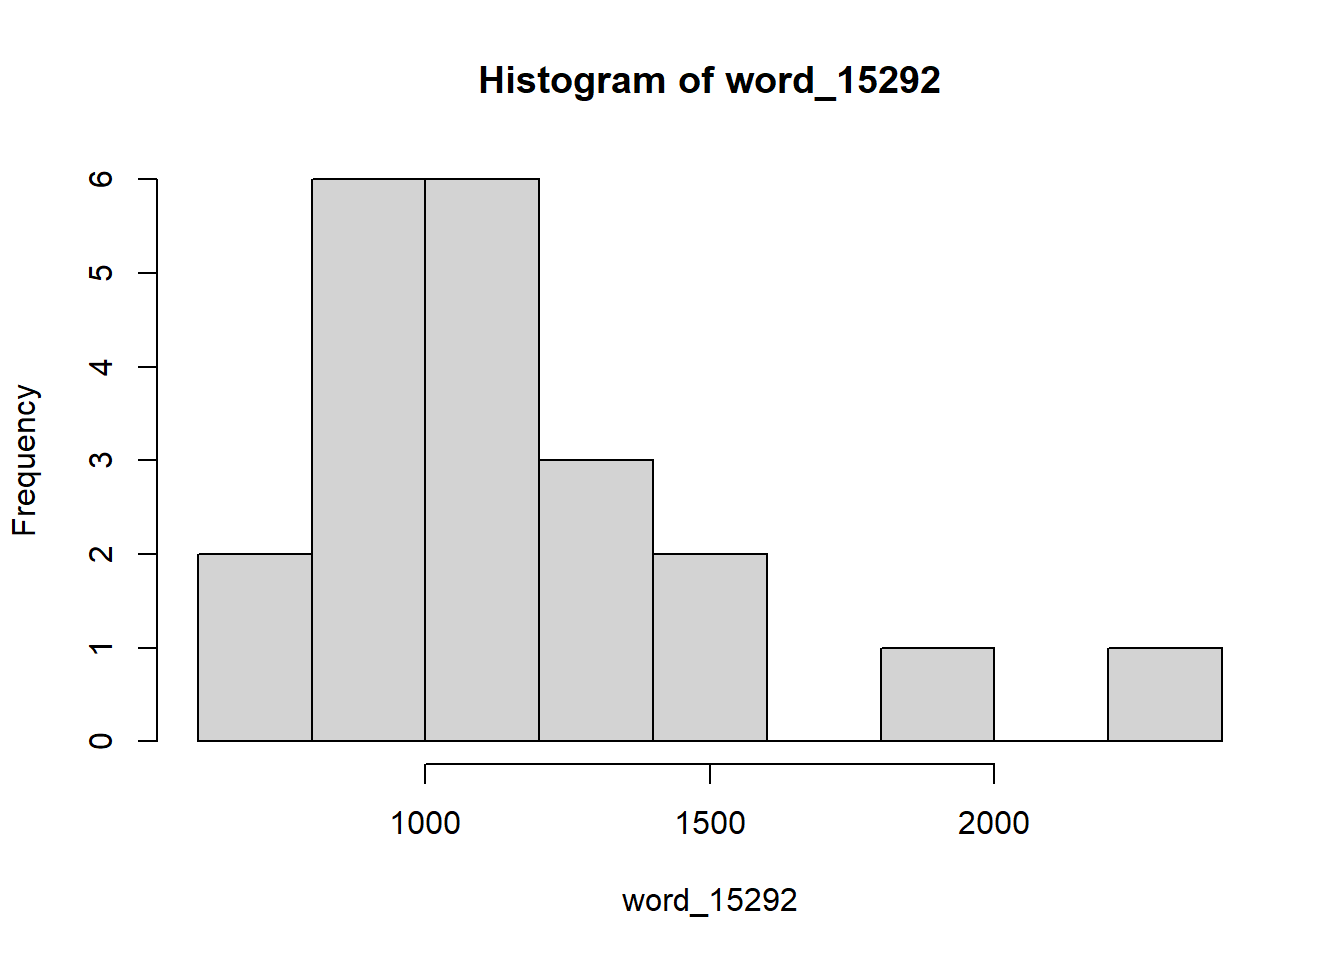
\includegraphics{assignment1_final_files/figure-latex/unnamed-chunk-6-1.pdf}

\begin{Shaded}
\begin{Highlighting}[]
\FunctionTok{hist}\NormalTok{(pseudoword\_15292)}
\end{Highlighting}
\end{Shaded}

\includegraphics{assignment1_final_files/figure-latex/unnamed-chunk-6-2.pdf}

\begin{Shaded}
\begin{Highlighting}[]
\CommentTok{\#square the values {-} not normal}
\NormalTok{sqrthist }\OtherTok{\textless{}{-}} \FunctionTok{sqrt}\NormalTok{(word\_15292)}
\FunctionTok{hist}\NormalTok{(sqrthist)}
\end{Highlighting}
\end{Shaded}

\includegraphics{assignment1_final_files/figure-latex/unnamed-chunk-6-3.pdf}

\begin{Shaded}
\begin{Highlighting}[]
\CommentTok{\#cube the values {-} not normal}
\NormalTok{cuberoot }\OtherTok{=} \ControlFlowTok{function}\NormalTok{(x) \{ }
     \ControlFlowTok{if}\NormalTok{(x }\SpecialCharTok{\textless{}} \DecValTok{0}\NormalTok{)}
\NormalTok{    \{ }\SpecialCharTok{{-}}\NormalTok{ (}\SpecialCharTok{{-}}\NormalTok{x)}\SpecialCharTok{\^{}}\NormalTok{(}\DecValTok{1}\SpecialCharTok{/}\DecValTok{3}\NormalTok{)\}}
    \ControlFlowTok{else}
\NormalTok{    \{x}\SpecialCharTok{\^{}}\NormalTok{(}\DecValTok{1}\SpecialCharTok{/}\DecValTok{3}\NormalTok{)\}}
\NormalTok{    \}}
\NormalTok{cubelist }\OtherTok{\textless{}{-}} \FunctionTok{sapply}\NormalTok{(word\_15292, cuberoot) }
\FunctionTok{print}\NormalTok{(cubelist)}
\end{Highlighting}
\end{Shaded}

\begin{verbatim}
##  [1] 13.017727 11.654500 10.489029 10.033223  9.528079  9.764497 10.412731
##  [8]  8.806572  9.359902 10.421946 10.160736 10.658957 10.803680  9.854562
## [15] 10.189712  9.244335  9.476396 12.402982 11.457309 11.186889  9.739963
\end{verbatim}

\begin{Shaded}
\begin{Highlighting}[]
\FunctionTok{hist}\NormalTok{(cubelist)}
\end{Highlighting}
\end{Shaded}

\includegraphics{assignment1_final_files/figure-latex/unnamed-chunk-6-4.pdf}

\begin{Shaded}
\begin{Highlighting}[]
\CommentTok{\#inverse the values {-} NORMAL}
\NormalTok{inverseList  }\OtherTok{\textless{}{-}} \FunctionTok{sapply}\NormalTok{(word\_15292, }\ControlFlowTok{function}\NormalTok{(x) }\DecValTok{1}\SpecialCharTok{/}\NormalTok{x)}
\FunctionTok{hist}\NormalTok{(inverseList)}

\NormalTok{pseudoinverseList  }\OtherTok{\textless{}{-}} \FunctionTok{sapply}\NormalTok{(pseudoword\_15292, }\ControlFlowTok{function}\NormalTok{(x) }\DecValTok{1}\SpecialCharTok{/}\NormalTok{x)}
\FunctionTok{hist}\NormalTok{(inverseList)}
\end{Highlighting}
\end{Shaded}

\includegraphics{assignment1_final_files/figure-latex/unnamed-chunk-6-5.pdf}

\begin{Shaded}
\begin{Highlighting}[]
\CommentTok{\#t and p values one{-}tailed}
\NormalTok{inverseT }\OtherTok{\textless{}{-}} \FunctionTok{tcalculation}\NormalTok{(inverseList, pseudoinverseList)}
\FunctionTok{print}\NormalTok{(inverseT)}
\end{Highlighting}
\end{Shaded}

\begin{verbatim}
## [1] -1.556482
\end{verbatim}

\begin{Shaded}
\begin{Highlighting}[]
\NormalTok{pval }\OtherTok{\textless{}{-}} \FunctionTok{pt}\NormalTok{(inverseT, }\AttributeTok{df=}\DecValTok{40}\NormalTok{, }\AttributeTok{lower.tail =} \ConstantTok{FALSE}\NormalTok{)}
\FunctionTok{print}\NormalTok{(}\FunctionTok{paste}\NormalTok{(}\StringTok{"T{-}value of the inversed data (one{-}tailed)"}\NormalTok{, }\FunctionTok{as.character}\NormalTok{(inverseT)))}
\end{Highlighting}
\end{Shaded}

\begin{verbatim}
## [1] "T-value of the inversed data (one-tailed) -1.55648217416487"
\end{verbatim}

\begin{Shaded}
\begin{Highlighting}[]
\FunctionTok{print}\NormalTok{(}\FunctionTok{paste}\NormalTok{(}\StringTok{"P{-}value of the inversed data (one{-}tailed)"}\NormalTok{, }\FunctionTok{as.character}\NormalTok{(pval)))}
\end{Highlighting}
\end{Shaded}

\begin{verbatim}
## [1] "P-value of the inversed data (one-tailed) 0.936264440798912"
\end{verbatim}

\hypertarget{q4-aggregating-data}{%
\subsubsection{Q4: aggregating data}\label{q4-aggregating-data}}

Even if we get a normal distribution of underlying data, we still did
not address the issue of independence. Are all RTs in our data set
independent? Clearly not. Participants tend to differ in reaction times
from each other and so there will be a dependence in reaction times of
each participant. The way to avoid it is to not work with raw data but
aggregations.

Commonly when running a t-test on experimental data, we aggregate the
dependent variable, e.g., RTs for words, per participant (that is, we
get just one measure per participant, its mean RT over words). We do the
same for pseudowords. Then, we calculate the t-value over these
aggregated measures and then we calculate p-values.

Do this for the dataset and report the results. Be careful in thinking
about the type of t-test. Is this paired or unpaired?

\emph{The type is t-test in paired, because participants see all words,
so the data is not independent. So we need one datapoint per
participant, for both normal and pseudowords. But while we do have met
the assumptions of the t-test, we do not have significant difference
between normal and pseudowords. This can mean that there is no
difference in reaction time between normal and pseudowords.}

\begin{Shaded}
\begin{Highlighting}[]
\CommentTok{\#use a paired t{-}test}

\FunctionTok{library}\NormalTok{(dplyr)}

\NormalTok{bySubject\_byWord }\OtherTok{\textless{}{-}}\NormalTok{ merged\_data  }\SpecialCharTok{\%\textgreater{}\%}
  \FunctionTok{group\_by}\NormalTok{(IsWord, Subject) }\SpecialCharTok{\%\textgreater{}\%}
  \FunctionTok{summarise}\NormalTok{(}
    \AttributeTok{MeanRT =} \FunctionTok{mean}\NormalTok{(RT, }\AttributeTok{na.rm =} \ConstantTok{TRUE}\NormalTok{),}
    \AttributeTok{SdRT =} \FunctionTok{sd}\NormalTok{(RT, }\AttributeTok{na.rm =} \ConstantTok{TRUE}\NormalTok{),}
    \AttributeTok{MinRT =} \FunctionTok{min}\NormalTok{(RT, }\AttributeTok{na.rm =} \ConstantTok{TRUE}\NormalTok{),}
    \AttributeTok{MaxRT =} \FunctionTok{max}\NormalTok{(RT, }\AttributeTok{na.rm =} \ConstantTok{TRUE}\NormalTok{),}
    \AttributeTok{n =} \FunctionTok{length}\NormalTok{(RT)}
\NormalTok{  )}
\end{Highlighting}
\end{Shaded}

\begin{verbatim}
## `summarise()` has grouped output by 'IsWord'. You can override using the
## `.groups` argument.
\end{verbatim}

\begin{Shaded}
\begin{Highlighting}[]
\NormalTok{normal\_words }\OtherTok{\textless{}{-}}\NormalTok{ bySubject\_byWord }\SpecialCharTok{\%\textgreater{}\%} \CommentTok{\#this is from chatGPT}
  \FunctionTok{filter}\NormalTok{(IsWord }\SpecialCharTok{==} \ConstantTok{TRUE}\NormalTok{) }\SpecialCharTok{\%\textgreater{}\%} \CommentTok{\#this is from chatGPT}
  \FunctionTok{pull}\NormalTok{(MeanRT) }\CommentTok{\#this is from chatGPT}


\NormalTok{pseudo\_words }\OtherTok{\textless{}{-}}\NormalTok{ bySubject\_byWord }\SpecialCharTok{\%\textgreater{}\%}
  \FunctionTok{filter}\NormalTok{(IsWord }\SpecialCharTok{==} \ConstantTok{FALSE}\NormalTok{)}\SpecialCharTok{\%\textgreater{}\%}
  \FunctionTok{pull}\NormalTok{(MeanRT)}

\CommentTok{\#perform paired t test}
\FunctionTok{print}\NormalTok{(}\FunctionTok{t.test}\NormalTok{(normal\_words, pseudo\_words,  }\AttributeTok{paired =} \ConstantTok{TRUE}\NormalTok{, }\AttributeTok{alternative =} \StringTok{"two.sided"}\NormalTok{))}
\end{Highlighting}
\end{Shaded}

\begin{verbatim}
## 
##  Paired t-test
## 
## data:  normal_words and pseudo_words
## t = -20.483, df = 220, p-value < 2.2e-16
## alternative hypothesis: true mean difference is not equal to 0
## 95 percent confidence interval:
##  -146.0339 -120.3982
## sample estimates:
## mean difference 
##       -133.2161
\end{verbatim}

\hypertarget{q6-a-pitfall-for-p-values}{%
\subsubsection{Q6: a pitfall for
p-values}\label{q6-a-pitfall-for-p-values}}

\begin{Shaded}
\begin{Highlighting}[]
\NormalTok{generate.t }\OtherTok{\textless{}{-}} \ControlFlowTok{function}\NormalTok{() \{}
    
\NormalTok{    mysample }\OtherTok{\textless{}{-}} \FunctionTok{rnorm}\NormalTok{(}\DecValTok{20}\NormalTok{, }\AttributeTok{mean=}\DecValTok{0}\NormalTok{, }\AttributeTok{sd=}\DecValTok{10}\NormalTok{)}
\NormalTok{    tvalue }\OtherTok{\textless{}{-}} \FunctionTok{mean}\NormalTok{(mysample)}\SpecialCharTok{/}\FunctionTok{sqrt}\NormalTok{((}\FunctionTok{var}\NormalTok{(mysample)}\SpecialCharTok{/}\DecValTok{20}\NormalTok{))}
\NormalTok{    tvalue}

\NormalTok{\}}
\end{Highlighting}
\end{Shaded}

Above, we calculated \(p\) values based on the assumption that there are
40 degrees of freedom, corresponding to the collection of 42 data points
(21 for word\_15292 and 21 for pseudoword\_15292; for each group the
degrees of freedom are 21-1, which makes 40 degrees of freedom in
total). In a way, we assume that the amount of data points were fixed
and it was only open what the values of the data points was.

However, it is quite common that researchers do not know in advance how
many participants they want to collect. Imagine the following situation:
we decided we would be collecting data for the whole day and then we
will stop and check the results. It happens so that on that day, there
was a 50\% probability that we would collect 12 responses (6 for words,
6 for pseudowords) and a 50\% probability that we would collect 42 data
points (21 for words and 21 for pseudowords). In our actual sample, we
happened to collect the latter amount (i.e., 42 data points) and we got
results as shown in word\_15292 and pseudoword\_15292. What would
\emph{then} be the p-value?

This is probably the most challenging question in this exercise. Here is
a hint how to approach it: above (in Section \emph{Using the
t-distribution to report p-values}), we saw that you can approximate
\(t\) distribution using simulation. However, in the case above, we only
approximated a \(t\) distribution for a single sample, which must have
consisted of 20 data points. Here, the situation is more complex for two
reasons: (i) we collect two samples and calculate t-values by comparing
them, (ii) it is given that the size of the samples is either 12
responses or 42 responses. This will complicate the simulation, but once
you create it, you can read off the p-value from it just as we did
above.

If you cannot calculate the value, try to at least reason about this: do
you think that the p-value will be smaller than in Q4? Or will it be
greater? In any case, note one very unintuitive aspect of p-values: they
are dependent on experimenters' intentions and hypothetical situations
(which might often not be explicitly stated, and might not even be
considered!).

*The p-value is a measure of the probability of observing a result as
extreme as, or more extreme than, what was actually observed, under the
assumption that the null hypothesis is true. A p-value of 0.021 suggests
that there is about a 2.1\% chance of observing a t-value as extreme as
2.517527 under the null hypothesis that there is no difference between
the groups (words and pseudowords).

Since 0.021 is less than 0.05, we reject the null hypothesis and
conclude a statistically significant difference between the reaction
times for words and pseudowords for subject 15292, with a confidence
level set at 95\% (alpha = 0.05). This conclusion is based on the
experimentation data and the simulation model. The fact that we obtained
a significant result in the simulation suggests that our experimental
design and the observed effect size are robust enough to be detected as
statistically significant, even when considering the uncertainty in
sample size.*

\begin{Shaded}
\begin{Highlighting}[]
\FunctionTok{set.seed}\NormalTok{(}\DecValTok{123}\NormalTok{)  }\CommentTok{\# Ensure reproducibility}
\NormalTok{n\_simulations }\OtherTok{\textless{}{-}} \DecValTok{2000}  \CommentTok{\# Number of simulations to perform}
\NormalTok{observed\_t\_value }\OtherTok{\textless{}{-}} \FloatTok{2.517527}  \CommentTok{\# The t{-}value we calculated for 15292}
\NormalTok{prob\_12\_responses }\OtherTok{\textless{}{-}} \FloatTok{0.5}  \CommentTok{\# Probability of collecting 12 responses}
\NormalTok{prob\_42\_responses }\OtherTok{\textless{}{-}} \FloatTok{0.5}  \CommentTok{\# Probability of collecting 42 responses}

\CommentTok{\# Perform simulations}
\NormalTok{t\_values }\OtherTok{\textless{}{-}} \FunctionTok{replicate}\NormalTok{(n\_simulations, \{}
\NormalTok{  sample\_size }\OtherTok{\textless{}{-}} \FunctionTok{ifelse}\NormalTok{(}\FunctionTok{runif}\NormalTok{(}\DecValTok{1}\NormalTok{) }\SpecialCharTok{\textless{}}\NormalTok{ prob\_12\_responses, }\DecValTok{6}\NormalTok{, }\DecValTok{21}\NormalTok{)  }\CommentTok{\# Choose sample size based on probability}
\NormalTok{  sample\_size}
  \FunctionTok{generate.t}\NormalTok{()}
\NormalTok{\})}

\CommentTok{\# Calculate the proportion of simulations with a t{-}value as extreme as or more extreme than the observed}
\NormalTok{simulated\_p\_value }\OtherTok{\textless{}{-}} \FunctionTok{mean}\NormalTok{(}\FunctionTok{abs}\NormalTok{(t\_values) }\SpecialCharTok{\textgreater{}=} \FunctionTok{abs}\NormalTok{(observed\_t\_value))}


\FunctionTok{mean}\NormalTok{(}\FunctionTok{abs}\NormalTok{(t\_values))}
\end{Highlighting}
\end{Shaded}

\begin{verbatim}
## [1] 0.831365
\end{verbatim}

\begin{Shaded}
\begin{Highlighting}[]
\FunctionTok{mean}\NormalTok{(}\FunctionTok{abs}\NormalTok{(observed\_t\_value))}
\end{Highlighting}
\end{Shaded}

\begin{verbatim}
## [1] 2.517527
\end{verbatim}

\begin{Shaded}
\begin{Highlighting}[]
\NormalTok{sample\_size }\OtherTok{\textless{}{-}} \FunctionTok{ifelse}\NormalTok{(}\FunctionTok{runif}\NormalTok{(}\DecValTok{1}\NormalTok{) }\SpecialCharTok{\textless{}}\NormalTok{ prob\_12\_responses, }\DecValTok{6}\NormalTok{, }\DecValTok{21}\NormalTok{)  }\CommentTok{\# Choose sample size based on probability}
\NormalTok{pval }\OtherTok{\textless{}{-}} \FunctionTok{pt}\NormalTok{(t\_values, }\AttributeTok{df=}\NormalTok{sample\_size, }\AttributeTok{lower.tail =} \ConstantTok{FALSE}\NormalTok{)}

\CommentTok{\# Output the simulated p{-}value}
\NormalTok{simulated\_p\_value}
\end{Highlighting}
\end{Shaded}

\begin{verbatim}
## [1] 0.021
\end{verbatim}

\hypertarget{q7-an-experiment-where-t-tests-work}{%
\subsubsection{Q7: an experiment where t-tests
work}\label{q7-an-experiment-where-t-tests-work}}

We raised various concerns regarding t-tests. We see that t-tests rely
on independence across responses, and they assume that responses are
distributed normally. The responses all have to follow the same normal
distribution. And we also saw that \(p\) values are hard to interpret,
they depend on (often unexpressed) intentions of the researcher.

But are there experiments for which t-tests are a great fit?

In this question, try to think of an ``experiment'\,' data which could
appropriately be analyzed by a t-test without any data aggregation. That
is, raw data are already suitable for a t-test analysis. Try to describe
the experiment in as much detail as possible: what conditions would
there be, what variables, which variable would function as a predictor,
which should be the outcome variable? Argue why you think t-tests are
suitable here (in particular, why you think the data are normal,
independent, identically distributed). The word experiment is put in
quotes, since you can think of an experiment very broadly -
observational studies (like checking a property of houses in a town, or
checking some property of students in a class) also qualifies as an
experiment.

\emph{Checking the high school entry exam results for students that were
taught by different teachers for a certain subject. In this way, we don'
t need to aggregate data, since per participant we will have only one
value, the exam score or percentage. We also assume that the groups are
of equal size. The performance on the exam for each participant should
be independent of others. Classes have usually over 30 students and a
teacher could teach 3 or 4 classes, so the sample would be big enough. A
two sample t-test should ideally be applied in this case, since we have
2 groups and we could consider the control group to be the one with the
usual teacher and the experimental one with a teacher that is just
starting teaching and is maybe using a different method.}

\hypertarget{q8-linear-models-and-graphical-representation}{%
\subsubsection{Q8: Linear models and graphical
representation}\label{q8-linear-models-and-graphical-representation}}

Run the models above (m1 and m2). Report results of both of them.

Then, provide a graphical summary accompanying m2. The summary should
show how Accuracy and IsWord affect RTs. In your plot we should be able
to see differences in the outcomes when the values of the predictor
changes. That is, we should be able to see that RTs change when the
values of IsWord change, and that RTs change when the values of ACC
change, and that IsWord and ACC interact in affecting RTs.

\begin{Shaded}
\begin{Highlighting}[]
\NormalTok{m1 }\OtherTok{\textless{}{-}} \FunctionTok{lm}\NormalTok{(RT }\SpecialCharTok{\textasciitilde{}}\NormalTok{ IsWord, merged\_data)}\CommentTok{\#put in your data here}
\FunctionTok{print}\NormalTok{(}\FunctionTok{summary}\NormalTok{(m1))}
\end{Highlighting}
\end{Shaded}

We can add more parameters and study how they affect the regression line
that predicts RTs. For example, the following model would consider the
effect of IsWord, Accuracy and their interaction. The * in the notation
calculates the main effect of both factors and the interaction of the
two factors.

\begin{Shaded}
\begin{Highlighting}[]
\NormalTok{m2 }\OtherTok{\textless{}{-}} \FunctionTok{lm}\NormalTok{(RT }\SpecialCharTok{\textasciitilde{}}\NormalTok{ IsWord }\SpecialCharTok{*}\NormalTok{ ACC, merged\_data)}\CommentTok{\#put in your data here}
\FunctionTok{print}\NormalTok{(}\FunctionTok{summary}\NormalTok{(m2))}

\CommentTok{\# The * sign signals interaction. See ?formula for details.}

\CommentTok{\# Load necessary libraries}
\FunctionTok{library}\NormalTok{(ggplot2)}

\CommentTok{\# Predict response times using model m2}
\NormalTok{predictions }\OtherTok{\textless{}{-}} \FunctionTok{expand.grid}\NormalTok{(}\AttributeTok{IsWord =} \FunctionTok{c}\NormalTok{(}\ConstantTok{FALSE}\NormalTok{, }\ConstantTok{TRUE}\NormalTok{), }\AttributeTok{ACC =} \FunctionTok{c}\NormalTok{(}\ConstantTok{FALSE}\NormalTok{, }\ConstantTok{TRUE}\NormalTok{))}
\NormalTok{predictions}\SpecialCharTok{$}\NormalTok{RT }\OtherTok{\textless{}{-}} \FunctionTok{predict}\NormalTok{(m2, }\AttributeTok{newdata =}\NormalTok{ predictions)}

\CommentTok{\# Plotting}
\FunctionTok{ggplot}\NormalTok{(predictions, }\FunctionTok{aes}\NormalTok{(}\AttributeTok{x =}\NormalTok{ ACC, }\AttributeTok{y =}\NormalTok{ RT, }\AttributeTok{color =} \FunctionTok{factor}\NormalTok{(IsWord))) }\SpecialCharTok{+}
  \FunctionTok{geom\_point}\NormalTok{() }\SpecialCharTok{+}
  \FunctionTok{geom\_line}\NormalTok{(}\FunctionTok{aes}\NormalTok{(}\AttributeTok{group =}\NormalTok{ IsWord), }\AttributeTok{linetype =} \StringTok{"dashed"}\NormalTok{) }\SpecialCharTok{+}
  \FunctionTok{labs}\NormalTok{(}\AttributeTok{x =} \StringTok{"Accuracy"}\NormalTok{, }\AttributeTok{y =} \StringTok{"Response Time"}\NormalTok{, }\AttributeTok{color =} \StringTok{"Is Word"}\NormalTok{) }\SpecialCharTok{+}
  \FunctionTok{theme\_minimal}\NormalTok{()}
\end{Highlighting}
\end{Shaded}

\hypertarget{q9-what-frequency-is-the-best-predictor}{%
\subsubsection{Q9: What frequency is the best
predictor?}\label{q9-what-frequency-is-the-best-predictor}}

There are various sources of frequency in our dataset: FreCOCA,
FreqGoogle, FreqSUBTLEX and FreqCOCAspok. These are frequencies of words
collected from four different corpora. Find out which of these provides
the best fit of the model to the log-transformed reaction times. You can
do so by comparing models in which different frequency sources are
added, or by comparing how big a proportion of the variance is explained
by the model.

After you find the answer, use the same frequency to address the
following observation: it has been claimed that log-frequency of a word
is a good predictor, better than a plain frequency, for log-reaction
times. Is this correct? Plot the relation between the outcome variable
and the non-transformed predictor variable to see whether any clear
relation can be observed and whether the relation looks linear. Then,
transform the frequency to log and plot again. Then, check the resulting
model.

Finally, check whether the log-transformation of all frequency data sets
changes your previous answer. Which corpus of frequency is now the best
predictor when we consider its log-transformation?

\begin{Shaded}
\begin{Highlighting}[]
\CommentTok{\# 1}
\CommentTok{\# Fit linear regression models using each frequency}
\NormalTok{model\_FreqCOCA }\OtherTok{\textless{}{-}} \FunctionTok{lm}\NormalTok{(}\FunctionTok{log}\NormalTok{(RT) }\SpecialCharTok{\textasciitilde{}}\NormalTok{ FreqCOCA,merged\_data)}
\NormalTok{model\_FreqGoogle }\OtherTok{\textless{}{-}} \FunctionTok{lm}\NormalTok{(}\FunctionTok{log}\NormalTok{(RT) }\SpecialCharTok{\textasciitilde{}}\NormalTok{ FreqGoogle, merged\_data)}
\NormalTok{model\_FreqSUBTLEX }\OtherTok{\textless{}{-}} \FunctionTok{lm}\NormalTok{(}\FunctionTok{log}\NormalTok{(RT) }\SpecialCharTok{\textasciitilde{}}\NormalTok{ FreqSUBTLEX,  merged\_data)}
\NormalTok{model\_FreqCOCAspok }\OtherTok{\textless{}{-}} \FunctionTok{lm}\NormalTok{(}\FunctionTok{log}\NormalTok{(RT) }\SpecialCharTok{\textasciitilde{}}\NormalTok{ FreqCOCAspok, merged\_data)}

\CommentTok{\# Compare values}
\NormalTok{rsquared\_values }\OtherTok{\textless{}{-}} \FunctionTok{tibble}\NormalTok{(}
  \AttributeTok{Source =} \FunctionTok{c}\NormalTok{(}\StringTok{"FreqCOCA"}\NormalTok{, }\StringTok{"FreqGoogle"}\NormalTok{, }\StringTok{"FreqSUBTLEX"}\NormalTok{, }\StringTok{"FreqCOCAspok"}\NormalTok{),}
  \AttributeTok{R\_squared =} \FunctionTok{c}\NormalTok{(}\FunctionTok{summary}\NormalTok{(model\_FreqCOCA)}\SpecialCharTok{$}\NormalTok{r.squared,}
                \FunctionTok{summary}\NormalTok{(model\_FreqGoogle)}\SpecialCharTok{$}\NormalTok{r.squared,}
                \FunctionTok{summary}\NormalTok{(model\_FreqSUBTLEX)}\SpecialCharTok{$}\NormalTok{r.squared,}
                \FunctionTok{summary}\NormalTok{(model\_FreqCOCAspok)}\SpecialCharTok{$}\NormalTok{r.squared)}
\NormalTok{)}

\CommentTok{\# Print R{-}squared values}
\FunctionTok{print}\NormalTok{(rsquared\_values)}
\end{Highlighting}
\end{Shaded}

\begin{verbatim}
## # A tibble: 4 x 2
##   Source       R_squared
##   <chr>            <dbl>
## 1 FreqCOCA      0.000728
## 2 FreqGoogle    0.00102 
## 3 FreqSUBTLEX   0.000662
## 4 FreqCOCAspok  0.000763
\end{verbatim}

\begin{Shaded}
\begin{Highlighting}[]
\CommentTok{\# 2}
\CommentTok{\# Biggest value for FreqGoogle =\textgreater{}}

\CommentTok{\# Plot relation between log{-}transformed RT and FreqGoogle}
\FunctionTok{ggplot}\NormalTok{(merged\_data, }\FunctionTok{aes}\NormalTok{(}\AttributeTok{x =}\NormalTok{ FreqGoogle, }\AttributeTok{y =} \FunctionTok{log}\NormalTok{(RT))) }\SpecialCharTok{+}
  \FunctionTok{geom\_point}\NormalTok{() }\SpecialCharTok{+}
  \FunctionTok{geom\_smooth}\NormalTok{(}\AttributeTok{method =} \StringTok{"lm"}\NormalTok{, }\AttributeTok{se =} \ConstantTok{FALSE}\NormalTok{) }\SpecialCharTok{+}
  \FunctionTok{labs}\NormalTok{(}\AttributeTok{x =} \StringTok{"FreqGoogle"}\NormalTok{, }\AttributeTok{y =} \StringTok{"Log{-}transformed RT"}\NormalTok{) }\SpecialCharTok{+}
  \FunctionTok{ggtitle}\NormalTok{(}\StringTok{"Relation between log RT and FreqGoogle"}\NormalTok{)}
\end{Highlighting}
\end{Shaded}

\begin{verbatim}
## `geom_smooth()` using formula = 'y ~ x'
\end{verbatim}

\includegraphics{assignment1_final_files/figure-latex/unnamed-chunk-12-1.pdf}

\begin{Shaded}
\begin{Highlighting}[]
\CommentTok{\# Transform FreqGoogle to log scale}
\CommentTok{\# merged\_data$log\_FreqGoogle \textless{}{-} log(merged\_data$FreqGoogle)}

\CommentTok{\# Plot relation between log{-}transformed RT and log{-}transformed FreqGoogle}
\FunctionTok{ggplot}\NormalTok{(merged\_data, }\FunctionTok{aes}\NormalTok{(}\AttributeTok{x =} \FunctionTok{log}\NormalTok{(FreqGoogle), }\AttributeTok{y =} \FunctionTok{log}\NormalTok{(RT))) }\SpecialCharTok{+}
  \FunctionTok{geom\_point}\NormalTok{() }\SpecialCharTok{+}
  \FunctionTok{geom\_smooth}\NormalTok{(}\AttributeTok{method =} \StringTok{"lm"}\NormalTok{, }\AttributeTok{se =} \ConstantTok{FALSE}\NormalTok{) }\SpecialCharTok{+}
  \FunctionTok{labs}\NormalTok{(}\AttributeTok{x =} \StringTok{"Log FreqGoogle"}\NormalTok{, }\AttributeTok{y =} \StringTok{"Log{-}transformed RT"}\NormalTok{) }\SpecialCharTok{+}
  \FunctionTok{ggtitle}\NormalTok{(}\StringTok{"Relation between log RT and log FreqGoogle"}\NormalTok{)}
\end{Highlighting}
\end{Shaded}

\begin{verbatim}
## `geom_smooth()` using formula = 'y ~ x'
\end{verbatim}

\begin{verbatim}
## Warning: Removed 86226 rows containing non-finite values (`stat_smooth()`).
\end{verbatim}

\includegraphics{assignment1_final_files/figure-latex/unnamed-chunk-12-2.pdf}

\begin{Shaded}
\begin{Highlighting}[]
\CommentTok{\# 3}
\CommentTok{\# this part doesn\textquotesingle{}t work yet}
\CommentTok{\# Fit linear regression models using each frequency }
\CommentTok{\# merged\_data$log\_FreqCOCA \textless{}{-} as.factor(log(merged\_data$FreqCOCA))}
\CommentTok{\# merged\_data$log\_FreqCOCA \textless{}{-} log(merged\_data$FreqCOCA)}
\NormalTok{merged\_data}\SpecialCharTok{$}\NormalTok{FreqCOCA }\OtherTok{\textless{}{-}} \FunctionTok{replace}\NormalTok{(merged\_data}\SpecialCharTok{$}\NormalTok{FreqCOCA, merged\_data}\SpecialCharTok{$}\NormalTok{FreqCOCA }\SpecialCharTok{==} \DecValTok{0}\NormalTok{, }\ConstantTok{NA}\NormalTok{)}
\NormalTok{merged\_data}\SpecialCharTok{$}\NormalTok{FreqGoogle }\OtherTok{\textless{}{-}} \FunctionTok{replace}\NormalTok{(merged\_data}\SpecialCharTok{$}\NormalTok{FreqGoogle, merged\_data}\SpecialCharTok{$}\NormalTok{FreqGoogle }\SpecialCharTok{==} \DecValTok{0}\NormalTok{, }\ConstantTok{NA}\NormalTok{)}
\NormalTok{merged\_data}\SpecialCharTok{$}\NormalTok{FreqSUBTLEX }\OtherTok{\textless{}{-}} \FunctionTok{replace}\NormalTok{(merged\_data}\SpecialCharTok{$}\NormalTok{FreqSUBTLEX, merged\_data}\SpecialCharTok{$}\NormalTok{FreqSUBTLEX }\SpecialCharTok{==} \DecValTok{0}\NormalTok{, }\ConstantTok{NA}\NormalTok{)}
\NormalTok{merged\_data}\SpecialCharTok{$}\NormalTok{FreqCOCAspok }\OtherTok{\textless{}{-}} \FunctionTok{replace}\NormalTok{(merged\_data}\SpecialCharTok{$}\NormalTok{FreqCOCAspok, merged\_data}\SpecialCharTok{$}\NormalTok{FreqCOCAspok }\SpecialCharTok{==} \DecValTok{0}\NormalTok{, }\ConstantTok{NA}\NormalTok{)}
\NormalTok{model\_logFreqCOCA }\OtherTok{\textless{}{-}} \FunctionTok{lm}\NormalTok{(}\FunctionTok{log}\NormalTok{(RT) }\SpecialCharTok{\textasciitilde{}} \FunctionTok{log}\NormalTok{(FreqCOCA) ,merged\_data, }\AttributeTok{na.action =} \StringTok{"na.omit"}\NormalTok{)}
\NormalTok{model\_logFreqGoogle }\OtherTok{\textless{}{-}} \FunctionTok{lm}\NormalTok{(}\FunctionTok{log}\NormalTok{(RT) }\SpecialCharTok{\textasciitilde{}}  \FunctionTok{log}\NormalTok{(FreqGoogle),merged\_data)}
\NormalTok{model\_logFreqSUBTLEX }\OtherTok{\textless{}{-}} \FunctionTok{lm}\NormalTok{(}\FunctionTok{log}\NormalTok{(RT) }\SpecialCharTok{\textasciitilde{}} \FunctionTok{log}\NormalTok{(FreqSUBTLEX), merged\_data)}
\NormalTok{model\_logFreqCOCAspok }\OtherTok{\textless{}{-}} \FunctionTok{lm}\NormalTok{(}\FunctionTok{log}\NormalTok{(RT) }\SpecialCharTok{\textasciitilde{}} \FunctionTok{log}\NormalTok{(FreqCOCAspok), merged\_data)}

\CommentTok{\# Compare values}
\NormalTok{rsquared\_values }\OtherTok{\textless{}{-}} \FunctionTok{tibble}\NormalTok{(}
  \AttributeTok{Source =} \FunctionTok{c}\NormalTok{(}\StringTok{"FreqCOCA"}\NormalTok{, }\StringTok{"FreqGoogle"}\NormalTok{, }\StringTok{"FreqSUBTLEX"}\NormalTok{, }\StringTok{"FreqCOCAspok"}\NormalTok{),}
  \AttributeTok{R\_squared =} \FunctionTok{c}\NormalTok{(}\FunctionTok{summary}\NormalTok{(model\_logFreqCOCA)}\SpecialCharTok{$}\NormalTok{r.squared,}
                \FunctionTok{summary}\NormalTok{(model\_logFreqGoogle)}\SpecialCharTok{$}\NormalTok{r.squared,}
                \FunctionTok{summary}\NormalTok{(model\_logFreqSUBTLEX)}\SpecialCharTok{$}\NormalTok{r.squared,}
                \FunctionTok{summary}\NormalTok{(model\_logFreqCOCAspok)}\SpecialCharTok{$}\NormalTok{r.squared)}
\NormalTok{)}

\CommentTok{\# Print R{-}squared values}
\FunctionTok{print}\NormalTok{(rsquared\_values)}
\end{Highlighting}
\end{Shaded}

\begin{verbatim}
## # A tibble: 4 x 2
##   Source       R_squared
##   <chr>            <dbl>
## 1 FreqCOCA        0.0545
## 2 FreqGoogle      0.0524
## 3 FreqSUBTLEX     0.0519
## 4 FreqCOCAspok    0.0406
\end{verbatim}

\begin{Shaded}
\begin{Highlighting}[]
\CommentTok{\# The answer to which corpus of frequency is now the best predictor when we consider its log{-}transformation is now FreqCOCA.}
\end{Highlighting}
\end{Shaded}

\hypertarget{q10-experiment-design}{%
\subsubsection{Q10: Experiment design}\label{q10-experiment-design}}

You are asked to design an experiment that will test whether log
frequency or plain frequency is the right predictor of log reaction
times (so, you basically want to test your answer to Q9, but rather than
using a corpus data, you want to test your answer in a novel
experiment). Your experiment should be a lexical decision task. What
will the design be like? Describe (i) the conditions in your
experiments, (ii) at least two items in your experiment (these should be
words used in the lexical decision task), (iii) what fillers and control
items you would use, (iv) how many stimuli would the whole experiment
consist of, (v) what log-frequency predicts and what plain frequency
predicts as results in your experiment.

*I asked chatGPT if verb vs noun was also a lexical decision task, but
that was not the case, so we chose for a traditional word vs nonword
task. I also asked chatGPT what log frequencies were and how that would
be a condition for a participant. Lastly I asked for a definition of
control and fillers, as I could not find a real definition from
literature.

\begin{enumerate}
\def\labelenumi{(\roman{enumi})}
\item
  The first factor is sentences with all words versus sentences
  containing words and one non word, the second factor is plain versus
  log frequency. But this still gives the participant 2 conditions when
  they perform the experiment, word and nonword. The other factor will
  be implemented in the data-analysis.
\item
  Some words are: ``This is an apple'' ``I love banana'' ``I do not own
  a house''
\end{enumerate}

Some non-words are: ``I would like some slsai'' ``plors are fun''
``sljdfl''

\begin{enumerate}
\def\labelenumi{(\roman{enumi})}
\setcounter{enumi}{2}
\tightlist
\item
  Fillers should distract the participant from the main purpose of the
  study, a filler would be a mathematical formula instead of words. A
  control should serve as a baseline, a control would be one word or one
  pseudoword, removed from the sentence.
\end{enumerate}

Marinis and Cunnings (2018) advise a ratio of at least 1:1 for critical
items versus fillers. Arehalli and Wittenberg (2020) presented a sample
of psycholinguistic and their number of stimuli. Most studies in the
sample had a number of critical items between 30-40. So if we were to
pick 35 critical items, with a filler ration of 1:1, that is 70 items +
35 control items, because we want to measure the control as well. That
is a total of 105 items per participant.

\begin{enumerate}
\def\labelenumi{(\alph{enumi})}
\setcounter{enumi}{21}
\tightlist
\item
  We then can see in the data-analysis if the plain frequencies are
  better predictors of log reaction time or of log frequencies are
  better predictors of log reaction time (that is, if it is a better
  predictor and a word is more frequent, then the reaction time should
  also change with it, like being shorter). We can see which predictors
  have significant relationships with the log reaction times. If the log
  frequencies have better predictive value of the log reaction times,
  then this would mean that it would be better for the model to have log
  frequencies. And the same with plain frequencies. *
\end{enumerate}

\hypertarget{bibliography}{%
\subsection{Bibliography}\label{bibliography}}

Tucker, Benjamin V, Daniel Brenner, D Kyle Danielson, Matthew C Kelley,
Filip Nenadic, and Michelle Sims. 2019. \emph{The massive auditory
lexical decision (MALD) database.} Behavior research methods
51:1187--1204.

\end{document}
